\section{Abstract folding}
\frame{\tableofcontents[currentsection]}

\begin{frame}{What kind of folding?}
    \pause
    There are many different kinds of folding (e.\,g. Origami)
    \pause
    Here:
    \begin{itemize}
        \pause
        \item Folding of surface in $\R^3$
        \pause
        \item Possible folding edges are fixed
        \pause
        \item Folding should be rigid (no curvature)
    \end{itemize}

    \pause
    Goal: Classify possible folding patterns (given a net)

    \pause
    \begin{center}
        \movie[ height = 0.4\textwidth, width = 0.4\textwidth, autostart, loop ]{}{TorusNetz.mp4}
    \end{center}

\end{frame}


\begin{frame}{Why are embeddings hard?}
    \pause
    Ideally, we would like to have embeddings.
    
    \pause
    But we want to define folding independently from an embedding, since:

    \begin{itemize}
        \pause
        \item They are very hard to compute (even for small examples)
        \pause
        \item We can only show foldability for specific small examples
            \begin{itemize}
                \pause
                \item Usually using regularity (like crystallographic symmetry)
                \pause
                \item No general method
            \end{itemize}
        \pause
        \item It is very hard to define iterated folding in an embedding
    \end{itemize}

    \pause
    \begin{center}
        \movie[ height = 0.4\textwidth, width = 0.4\textwidth, autostart, loop ]{}{TorusNetz.mp4}
    \end{center}

\end{frame}

%TODO what about forced folding? Or closedness of surfaces under folding? RETHINK this

\begin{frame}{Is there an alternative?}
    \pause
    Central idea:
    \begin{itemize}
        \pause
        \item Don't model folding process (needs embedding)
        \pause
        \item Describe starting and final folding state
            \begin{itemize}
                \pause
                \item Only consider changes in the topology
                    \pause (like identification of faces)
                \pause
                \item allows abstraction from embedding
            \end{itemize}
    \end{itemize}

    % Use pentagon-flippy to illustrate incidence rigidity

    \pause
    $\leadsto$ Incidence geometry (polygonal complex/surface)

    \begin{itemize}
        \pause
        \item Captures some folding restrictions \pause (rigidity of tetrahedron)
        \pause
        \item Still needs a lot of refinement
    \end{itemize}
\end{frame}


\begin{frame}{Important properties of folding}
    \begin{itemize}
        \item<2-> The class of surfaces is not closed under folding
        \item<3-> Folding can be undone by \textit{unfolding}
        \item<4-> Identification of two faces might force identification of two other faces
            \begin{itemize}
                \item<7-> Can apply to arbitrary many faces 
                \item<10-> The forced identification is not unique
                \item<14->[$\Rightarrow$] Identify only two faces at a time
            \end{itemize}
    \end{itemize}

    \begin{overlayarea}{\textwidth}{0.3\textwidth}
        \begin{center}
            \only<5-7|handout:0>{
                % First identification
                \begin{tikzpicture}
                    \def\Hdist{1.5}
	    	    \def\Vdist{1}
			
		    \coordinate (A) at (-\Hdist,0);
		    \coordinate (B) at (0,\Vdist);
		    \coordinate (C) at (\Hdist,0);
		    \coordinate (D) at (0,-\Vdist);
                    \draw (A) -- (B) -- (C) -- (D) -- cycle;

		    \foreach \p in {A,B,C,D}
		        \fill [\vertexColor] (\p) circle (1.5pt);
		    \draw [<->,red,thick] ($(B)!0.5!(A)$) -- ($(D)!0.5!(A)$);
                    \uncover<6-7>{
                        \draw[<->,red,thick] ($(B)!0.5!(C)$) -- ($(D)!0.5!(C)$);
                    }
                \end{tikzpicture}
            }

            % Arbitrary many faces
            \only<8-10|handout:0>{
                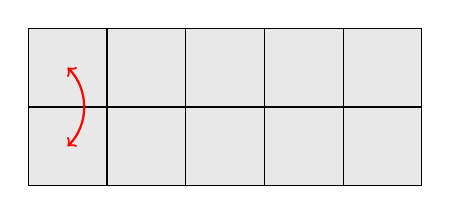
\begin{tikzpicture}
		    \foreach \i/\j in {1/0, 2/1, 3/2, 4/3, 5/4}
		    {
		        \filldraw [fill=black!9!white] (\j,0) -- (\i,0) -- (\i,1) -- (\j,1) -- cycle;
		        \filldraw [fill=black!9!white] (\j,0) -- (\i,0) -- (\i,-1) -- (\j,-1) -- cycle;
		    }
                    \uncover<9-10>{
                        \draw [red,<->,thick] (0.5,0.5) to [out=-45,in=45] (0.5,-0.5);
	            }
                \end{tikzpicture}
            }

            %TODO picture of non-uniqueness:
            % 11: general picture
            % 12: First possible fold
            % 13: Second possible fold

            % Anomaly-picture
            \only<15-|handout:1>{
                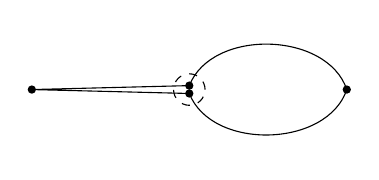
\begin{tikzpicture}
		    \def\r{2}	
		    \def\eps{0.05}
				
		    \coordinate (A) at (-\r,0);
		    \coordinate (B) at (0,\eps);
		    \coordinate (C) at (\r,0);
		    \coordinate (D) at (0,-\eps);
			
		    \draw (D) -- (A) -- (B);
		    \draw (B) to [bend left=70] (C);
		    \draw (D) to [bend right=70] (C);
			
		    \foreach \point in {A,B,C,D}
		        \fill [\vertexColor] (\point) circle (1.5pt);
				
		    \draw [dashed] (0,0) circle (0.2);
                \end{tikzpicture}
            }
        \end{center}
    \end{overlayarea}
\end{frame}


\begin{frame}{How to define abstract folding?}
    \uncover<2->{We need to define two structures:}
    \begin{enumerate}
        \item<3-> A folding state
            \begin{itemize}
                \item<5-> Based on polygonal complexes
                \item<6-> Describe ``is folded together" by an equivalence relation
                \item<7-> Describe order of faces in folding state
            \end{itemize}
        \item<4-> The folding steps
            \begin{itemize}
                \item<8-> Only two faces at a time
                \item<9-> Explain ``unordered folding" (e.\,g. covering)
                \item<10-> Modify to include face order relations
            \end{itemize}
    \end{enumerate}
\end{frame}


\begin{frame}{Unordered Folding (Covering)}
    \begin{center}
        \begin{tikzpicture}
            \def\xOff{1.8}
            \def\yOff{1.5}

            %     B
            %   / | \
            % A   |   C
            %   \ | /
            %     D
            \coordinate (A) at (-\xOff,0);
            \coordinate (B) at (0,\yOff);
            \coordinate (C) at (\xOff,0);
            \coordinate (D) at (0,-\yOff);

            \uncover<3->{
                \filldraw[face] (A) -- (B) -- (D) -- cycle;
                \node at (barycentric cs:A=1,B=1,D=1) {$I$};
                \filldraw[face] (B) -- (C) -- (D) -- cycle;
                \node at (barycentric cs:B=1,C=1,D=1) {$II$};

                \foreach \p in {A,B,C,D}
                    \fill[\vertexColor] (\p) circle (1.5pt);
            }

            \uncover<5-7|handout:1>{
                \draw[red,thick,->] (barycentric cs:A=1,B=2,D=2) to[bend left] (barycentric cs:B=2,C=1,D=2);
                \draw[red,thick,->] ($(A)!0.5!(B)$) to[bend right] ($(B)!0.5!(C)$);
                \draw[red,thick,->] ($(A)!0.5!(D)$) to[bend left] ($(D)!0.5!(C)$);
            }
        \end{tikzpicture}
    \end{center}

    \begin{overprint}
        \onslide<1-7|handout:1>
        
        \uncover<2-7>{
            Why do we need more than a polygonal complex?
        }

        \uncover<4-7>{
            Naive folding definition: surjective map that respects incidence
        }

        \uncover<6-7>{
            Problem: Can't be unfolded
        }

        \uncover<7>{
            $\Rightarrow$ Folding state should not forget original structure
        }


        \onslide<8-16|handout:2>

        \uncover<8-16>{
            Represent folding by equivalence relation
            \begin{itemize}
                \item<9-> Separate relation on vertices, edges and faces
                \item<10-> Two elements are equivalent if they are folded together
                \item<11-> If two edges are equivalent, 
                    \uncover<12->{then their vertices have to be as well}
                    \uncover<13->{(likewise for faces)}
                \item<14-> The vertices of an edge are not equivalent
                    \uncover<15->{(likewise for faces)}
                \item<16->[$\Rightarrow$] Unordered folding is coarsening of equivalence relation
            \end{itemize}
        }
    \end{overprint}
\end{frame}


\begin{frame}{How does folding work?}
    \begin{enumerate}
        \item<2-> Choose two faces that are not folded together
        \item<4-> Choose how to identify them \uncover<6->{(like $I \sim II$ and $1 \sim 4$)}
        \item<7-> Add those pairs to the equivalence relation
    \end{enumerate}

    \begin{center}
        \begin{tikzpicture}
            \def\xOff{1.8}
            \def\yOff{1.5}

            %     B
            %   / | \
            % A   |   C
            %   \ | /
            %     D
            \uncover<3->{
                \coordinate[label={[vertex]left:1}] (A) at (-\xOff,0);
                \coordinate[label={[vertex]above:2}] (B) at (0,\yOff);
                \coordinate[label={[vertex]right:4}] (C) at (\xOff,0);
                \coordinate[label={[vertex]below:3}] (D) at (0,-\yOff);

                \filldraw[face] (A) -- (B) -- (D) -- cycle;
                \node at (barycentric cs:A=1,B=1,D=1) {$I$};
                \filldraw[face] (B) -- (C) -- (D) -- cycle;
                \node at (barycentric cs:B=1,C=1,D=1) {$II$};

                \foreach \p in {A,B,C,D}
                    \fill[\vertexColor] (\p) circle (1.5pt);
            }

            \uncover<5->{
                \draw[red,thick,->] (barycentric cs:A=1,B=2,D=2) to[bend left] (barycentric cs:B=2,C=1,D=2);
                \draw[red,thick,->] ($(A)!0.5!(B)$) to[bend right] ($(B)!0.5!(C)$);
                \draw[red,thick,->] ($(A)!0.5!(D)$) to[bend left] ($(D)!0.5!(C)$);
            }
        \end{tikzpicture}
    \end{center}

    \uncover<8->{Restriction:}

    \uncover<9->{Two vertices in an edge can't be identified}
    \uncover<10->{(slightly generalized)}
\end{frame}


\begin{frame}{Restrictions of unordered folding}
    \pause
    We can't work with ordering of faces:
    \pause
    \begin{center}
        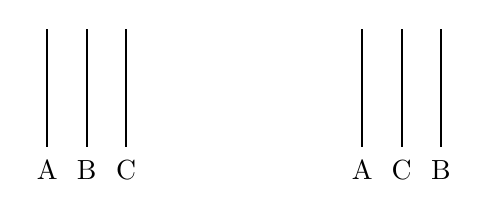
\begin{tikzpicture}
            \def\len{1.5}
            \def\xOff{0.5}
            \def\nOff{-0.3}
            \def\wid{thick}

            \draw[\colA,\wid] (0,0) -- (0,\len);
            \node[\colA] at (0,\nOff) {A};

            \draw[\colB,\wid] (\xOff,0) -- (\xOff,\len);
            \node[\colB] at (\xOff,\nOff) {B};

            \draw[\colC,\wid] (2*\xOff,0) -- (2*\xOff,\len);
            \node[\colC] at (2*\xOff,\nOff) {C};


            % Second lines
            \begin{scope}[xshift=4cm]
                \draw[\colA,\wid] (0,0) -- (0,\len);
                \node[\colA] at (0,\nOff) {A};

                \draw[\colC,\wid] (\xOff,0) -- (\xOff,\len);
                \node[\colC] at (\xOff,\nOff) {C};

                \draw[\colB,\wid] (2*\xOff,0) -- (2*\xOff,\len);
                \node[\colB] at (2*\xOff,\nOff) {B};
            \end{scope}
        \end{tikzpicture}
    \end{center}

    \pause
    Adding a linear order on each face equivalence class
    \pause is not enough:
    \pause
    \begin{center}
        \begin{tikzpicture}
            \def\len{1}
            \def\nScale{1.3}
            \def\wid{thick}

            \draw[\colA,\wid] (0,0) -- (210:\len);
            \node[\colA] at (210:\nScale*\len) {A};

            \draw[\colB,\wid] (0,0) -- (-30:\len);
            \node[\colB] at (-30:\nScale*\len) {B};

            \draw[\colC,\wid] (0,0) -- (90:\len);
            \node[\colC] at (90:\nScale*\len) {C};

            \fill (0,0) circle (1.5pt);

            \begin{scope}[xshift=4cm]
                \draw[\colA,\wid] (0,0) -- (210:\len);
                \node[\colA] at (210:\nScale*\len) {A};

                \draw[\colC,\wid] (0,0) -- (-30:\len);
                \node[\colC] at (-30:\nScale*\len) {C};

                \draw[\colB,\wid] (0,0) -- (90:\len);
                \node[\colB] at (90:\nScale*\len) {B};

                \fill (0,0) circle (1.5pt);
            \end{scope}
        \end{tikzpicture}
    \end{center}

    \pause
    $\leadsto$ define order of faces around edges
    \pause
    (we will skip the details)
\end{frame}


\begin{frame}{Folding complex}
    \pause
    \begin{defi}
        A \textbf{folding complex}
        \pause
        is a polygonal complex together with
        \begin{enumerate}
            \pause
            \item An equivalence relation on vertices, edges and faces
                \pause (``is folded together")
            \pause
            \item A linear ordering on each face equivalence class
            \pause
            \item A cyclical ordering of the faces around each edge equivalence class
        \end{enumerate}
        \pause
        such that the orderings are compatible
        \pause
        (in an appropriate sense).
    \end{defi}

    \pause
    To identify faces with each other, we have to combine those orderings.
    \begin{itemize}
        \pause
        \item linear orderings get concatenated
        \pause
        \item cyclical orderings are opened at one point
            \pause
            and combined
        \pause
        \item[!!] compatibility is not easily transfered,
            \pause
            but can be calculated
    \end{itemize}

\end{frame}


\begin{frame}{Changed definition of folding}
    \begin{overprint}
        \only<2-4|handout:0>{Before (no ordering):}
        \only<5-> Folding with ordering:
    \end{overprint}

    \begin{enumerate}
        \item<3-> Choose two faces that are not folded together
        \item<4-> Choose how to identify them and extend the equivalence relation
        \item<9-> Choose the sides of the faces that will meet
            \uncover<10-> and modify the orderings
    \end{enumerate}

    \uncover<6->{
        $\leadsto$ Each face has two sides
    }

    \begin{center}
        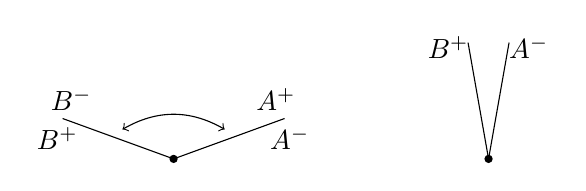
\begin{tikzpicture}
            \def\len{1.5}
            \def\wA{20}
            \def\wB{160}
            \def\nOff{10}

            \uncover<7->{
                \draw[\colA] (0,0) -- (\wA:\len);
                \node[\colA] at (\wA+\nOff:\len) {$A^+$};
                \node[\colA] at (\wA-\nOff:\len) {$A^-$};

                \draw[\colB] (0,0) -- (\wB:\len);
                \node[\colB] at (\wB+\nOff:\len) {$B^+$};
                \node[\colB] at (\wB-\nOff:\len) {$B^-$};

                \fill (0,0) circle (1.5pt);
            }

            \uncover<8->{
                \draw[<->] (\wB-\nOff: 0.5*\len) to[bend left] (\wA+\nOff:0.5*\len);
            }

            \begin{scope}[xshift=4cm]
                \uncover<8->{
                    \def\wA{80}
                    \def\wB{100}
                    
                    \draw[\colA] (0,0) -- (\wA:\len);
                    \node[\colA] at (\wA-\nOff:\len) {$A^-$};

                    \draw[\colB] (0,0) -- (\wB:\len);
                    \node[\colB] at (\wB+\nOff:\len) {$B^+$};

                    \fill (0,0) circle (1.5pt);
                }
            \end{scope}

        \end{tikzpicture}
    \end{center}


    
\end{frame}



